\documentclass[11pt]{article} %This sets the font size and the document class of your report. In this case we use 'article' as that is ideal for shorter reports.
\usepackage{amssymb}
\usepackage{amsmath}

% LaTeX can be enhanced by the use of packages. These packages can do many things, a few of the most common and useful are used here. They are declared before the document proper, in what is known as the 'preamble'. Packages need to be installed when a .tex file compiles into a .pdf, but should do so automatically.

\usepackage[top=2.54cm, bottom=2.54cm, left=2.75cm, right=2.75cm]{geometry} %This sets the margins of the report.

\usepackage{graphicx} % A package allowing insertion of images into the text.

\usepackage[linesnumbered,ruled,vlined]{algorithm2e}

% Choose your citations style by commenting out one of the following groups. If you decide to change style, you should also delete the .bbl file that you will find in the same folder as your .tex and .pdf files.

% IEEE style citation:
\usepackage[style=ieee]{biblatex}
\addbibresource{sem_1_report.bib}

%% Author-date style citation:
%\usepackage[round]{natbib} % A package that creates references in the author-date style, with round brackets
%\renewcommand{\cite}{\citep} % For use with natbib only: comment out for the cite package.
%\bibliographystyle{plainnat} % Author-date referencing (use in conjunction with the natbib package)
\usepackage{color} % Allows the colour of the font to be changed by using the '\color' command: This is just to support the blue comments in this template...use standard (black) text in your report.
\usepackage{float}
\linespread{1} % Sets the spacing between lines of text.
\setlength{\parindent}{0cm}  % Suppresses indentation of text at the start of a paragraph
\pagenumbering{arabic} % sets the style of page numbering for the report


\begin{document} % This begins the document proper and ends the pre-amble

% The last } finishes the chunk of text opening with {\color{blue}..., so all of the above appears as blue text. A common LaTeX error is to forget to close such a chunk of text, so if the formatting goes wrong look for a missing }.

% To get rid of the blue text, select and delete everything from '{\color' to '}', inclusive, leaving \ begin{titlepage} as the first command  after \begin{document}

\begin{center} % Starts the beginning of an environment where all text is centered.

{\Huge Simulating light detection in liquid argon time projection chambers for neutrino and dark matter experiments with deep learning techniques}\\[0.5cm] % [0.5cm] sets the distance between this line and the next.
\vspace{5mm}
\textit{Enrico Zammit Lonardelli}
\\
\vspace{5mm}
\text{9910821}
\\
\vspace{5mm}
\text{School of Physics and Astronomy}
\\
\vspace{5mm}
\text{The University of Manchester}
\\
\vspace{5mm}
\text{Masters Project}
\\
\vspace{5mm}
\text{December 2019}
\\
\vspace{5mm}
This experiment was performed in collaboration with \textit{Krishan Jethwa}\\[0.3cm] % The '\\' starts a new paragraph, and will only work after a paragraph has started, unless we use '~'.

% If this was an individual report then remove the "For an individual report" section and replace "Partner name".

\end{center}
\vspace{60mm}
{\Large \textbf{Abstract}}
\vspace{2mm}
\\
This report is a summary of the work that has been carried out in the first twelve weeks of our masters project. The aim was to investigate the ability of deep neural network methods to replace Geant4 Montecarlo simulations of LArTPCs. In this report we show a basic quantitative comparison between simulations carried out with Geant4 and the output of a Generative Adverserial Network (GAN). Finally, we successfully trained and tested 1D and 2D conditional GANs on the variables $S1$, $S2$ and $f_{200}$.
\pagebreak
% New paragraphs can either be initiated by a double vertical space i.e. tapping the enter button twice, which causes the paragraph below to be indented, or by a '\\', which does not cause the next paragraph to indent. In a long section of mainly writing, indentations on paragraphs can help break up the text into different sections. To avoid indentations in your report when they are not needed, use the  command before the line.

\section{Introduction}

\begin{figure}[H]
\centering
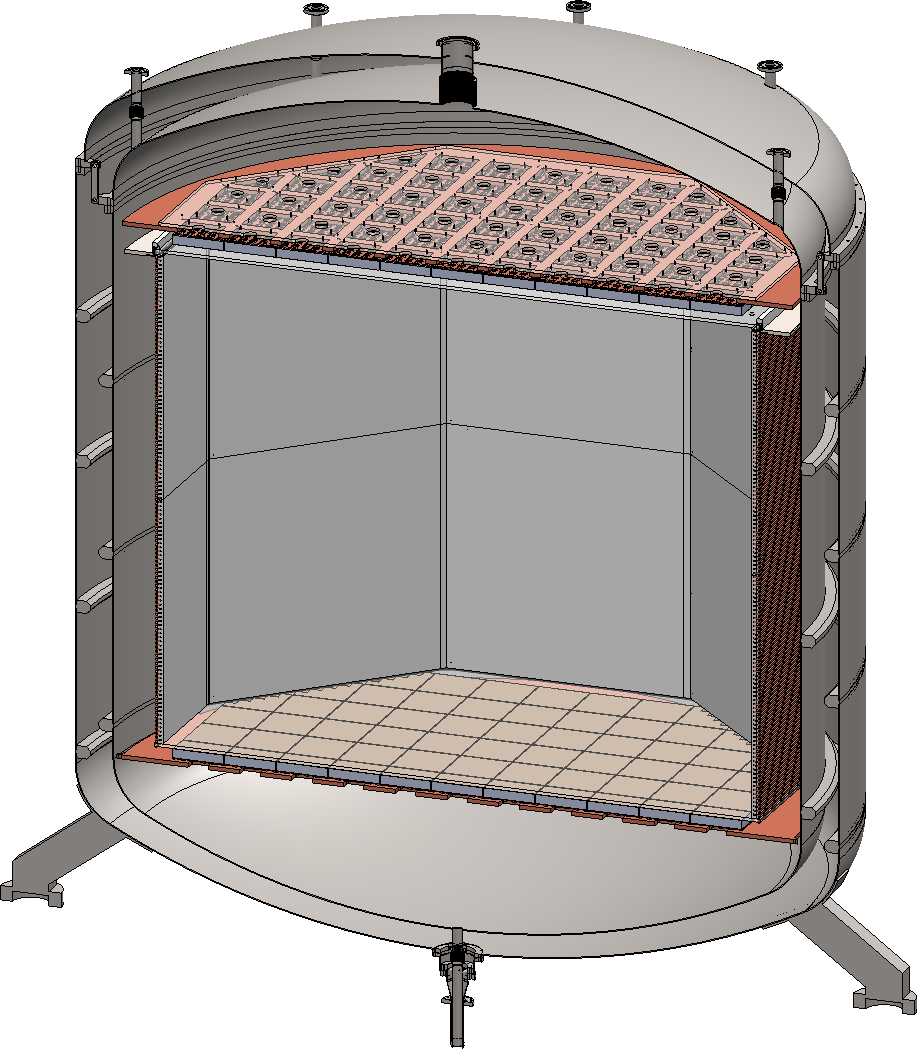
\includegraphics[scale=0.2]{images/LArTPC_diagram.png}
\caption{\cite{Aalseth_2018} 3D rendering of the Darkside20k LArTPC and surrounding cryostat.}
\label{fig:lartpc}
\end{figure}

Most modern neutrino and dark matter direct detection experiments make use of multi-tonne cryogenic noble liquid detector technologies \cite{rubbia1977liquid} \cite{Acciarri_2015} \cite{Chepel_2013}.
When a dark matter or neutrino interacts with the noble liquid atoms they cause recoils which produce scintillation. The current dark matter candidates are Weakly Interacting Massive Particles (WIMPs) \cite{pagani2017direct} and are the focus of most liquid noble gas TPCs. In order to actually interpret the light signals recorded in such experiments precise simulations of these detectors have been created \cite{Agnes_2017} and simulation models are calibrated to measured quantities such as the optical properties of cold noble liquids and photosensor efficiency.
\newline

The inherent problems that come with detail and complexity in simulations are the need for large computational resources and long processing times. The former are expensive but more importantly limit the use of simulation to the extent that models can be tuned to calibration data. The problem with the latter is that applying a small modification to the theory or running a different set of configurations means waiting a long time to get the results which might hinder what gets tried and tested within a collaboration.
\newline

As a result, an alternative approach is required to derive an accurate, fast but flexible simulation of noble liquid detectors that uses the experimental data directly to learn the model that best represents reality. This is why machine learning and deep neural networks are appealing as potential candidates.

\subsection{DarkSide 20k}
\subsubsection{The detector}
\begin{figure}[H]
\centering
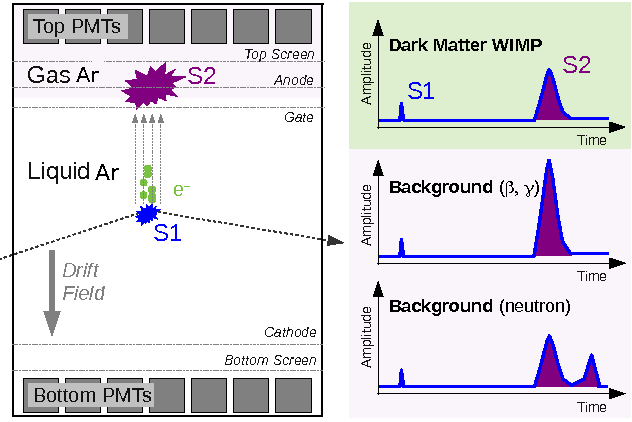
\includegraphics[scale=0.7]{images/tpc1.png}
\caption{\cite{PhysRevLett.119.181301} Schematic of the inner part of the LAr TPC showing background and signal intensities. Noting the much larger $S2$ in background, electron recoils (background) are discriminated from nuclear recoils (signal) by plotting the logarithm of the scintillation intensities against primary scintillation.}
\label{fig:s1s2}
\end{figure}

The DarkSide collaboration is planning on building a new Liquid Argon Time Projection Chamber (LArTPC) with 20t target mass after fiducial cuts \cite{Aalseth_2018} (called DarkSide-20k) located at Laboratori Nazionali del
Gran Sasso between 2020 and 2021. Figure \ref{fig:lartpc} shows a 3D illustration of the inner part of the detector . The outermost shell is a cryostat to keep the noble gas inside the chamber at liquid state. The liquid phase is chosen so as to create a very dense volume to maximise collision crossections between argon atoms and dark matter or neutrinos. The element is chosen to be noble so as to be electrically and chemically inert so that any drifting electrons produced from collisions are not absorbed by other argon atoms before detection.
\newline

When a WIMP enters the chamber it might recoil with an argon nucleus thus creating a primary scintillation known as \textbf{$S1$}. This will produce ionization electrons which will drift upwards in the liquid (due to an electric field) where there is a thin layer of argon in the gaseous phase. Here, the electrons will ionise the gas and produce a secondary scintillation known as \textbf{$S2$}. The electrons will then drift upwards and detected by transparent anode strips to measure timing signals for third dimension reconstruction. The photons will be detected by a multitude of silicon photon multipler tubes (SiPM) which will create a larger signal so as to be detected.
\newline

Figure \ref{fig:s1s2} shows the relative SiPM responses for $S1$ and $S2$ which will then be used in analysis to differentiate between signal (nuclear recoil) and background (electron recoil). Background has a much larger ratio of $S2$ to $S1$ so plotting the logarithm of the scintillation intensities against primary scintillation for the observed $S1$ and $S2$ produces a method of discrimination between signal and background.

\subsubsection{G4DS}
\begin{figure}[H]
\centering
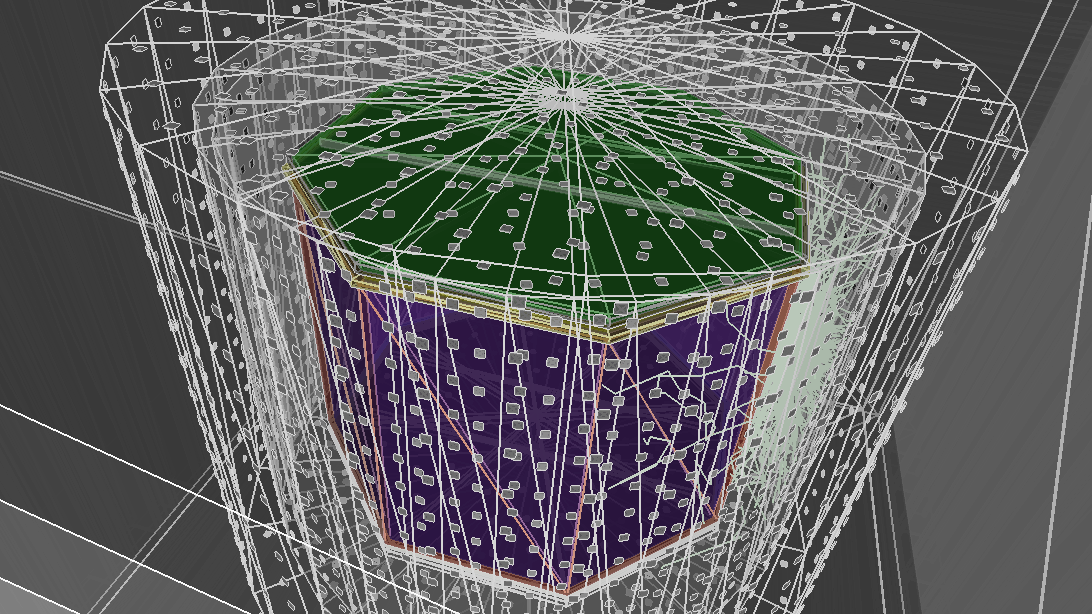
\includegraphics[scale=0.3]{images/config11.png}
\caption{A 3D visualisation of the configuration 11 used in our runs. Silicon photomultipliers can be seen in all the veto volumes together with the octagonal shape of the chamber.}
\label{fig:config11}
\end{figure}


Simulations for the complete detector are all carried out in a simulation software package called Geant4 \cite{G4}. After setting all physics packages and constants such as materials, dimensions and particles G4 will in turn carry out all Montecarlo simulations as required.
The DarkSide collaboration have their own G4 collection of macros, setups and configurations called G4DS and the results of these simulations are what we use as \textit{ground truth} for our machine learning models described later on. For the sake of this report and our work in these 12 weeks we have cloned a repository from the collaboration's \textit{Gitlab} account and used the branch called \textit{sol\_niamh\_andrzej\_g410.1.2} as our starting point.
The configuration macro used is 11 which is visualised in Figure \ref{fig:config11} and describes the current (to the time of writing this report) full setup of the detector with all SiPMs, argon buffers and vetoes.
\newline

Each run macro of the detector simulations is divided into three parts. The \textbf{Manager} which sets constants such as what is saved, how many events per run etc. The \textbf{Detector} which sets constants such as dimensions of the cryostat and chamber, and which preset detector configuration (eg. Veto chamber on/off) to run. The \textbf{Generator} which sets details of what particle to fire and where (eg. An argon atom recoil at a random position). We have run Ar40 recoils (which represents dark matter candidate events) at random positions and directions.
\newline

\begin{figure}[H]
\centering
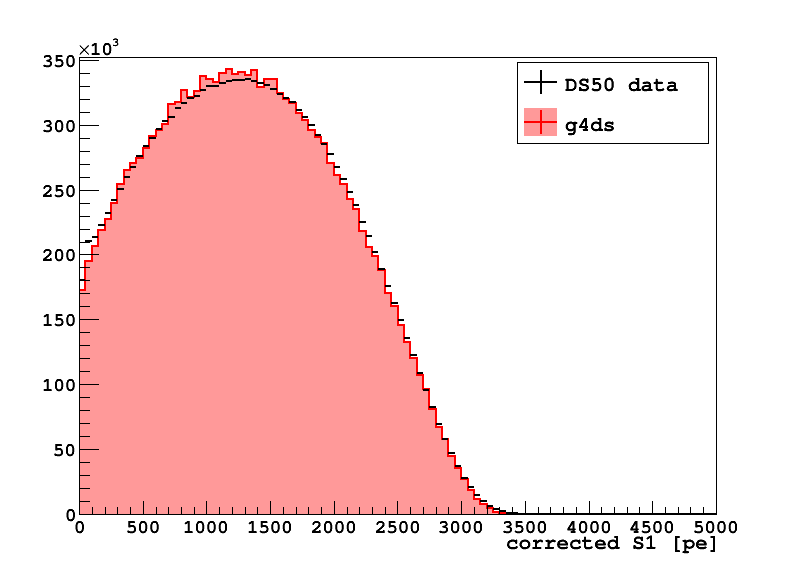
\includegraphics[scale=0.25]{images/s1_response.png}
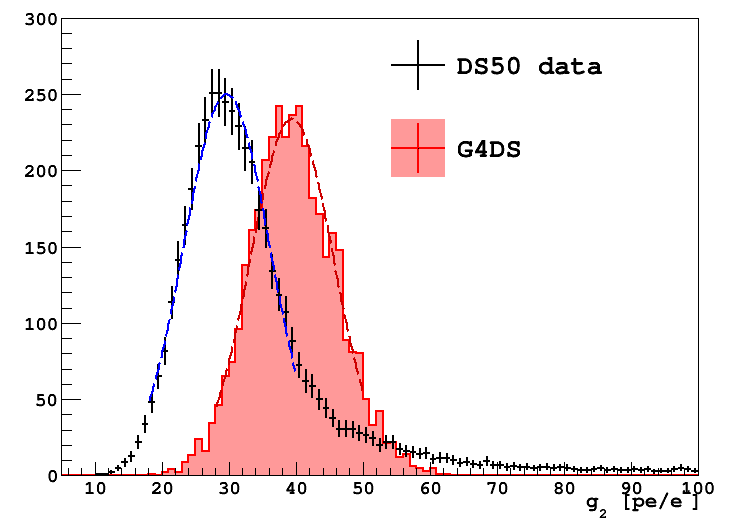
\includegraphics[scale=0.25]{images/s2_response.png}
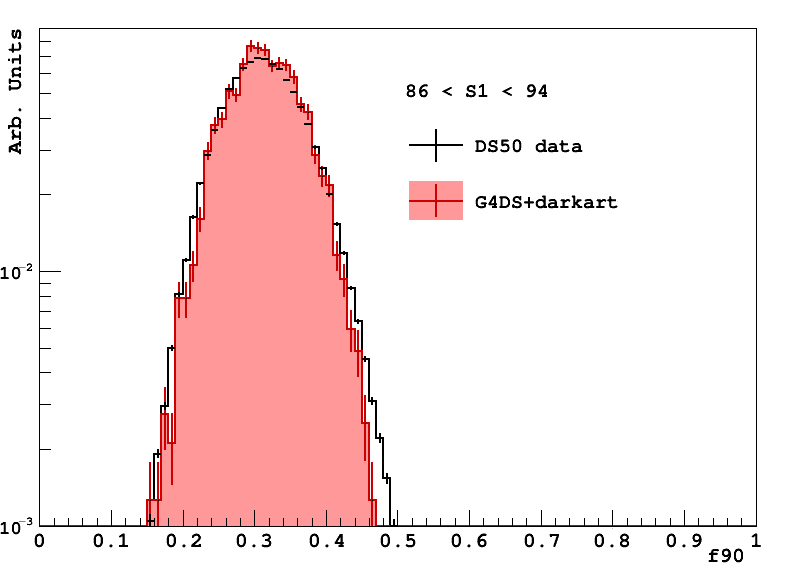
\includegraphics[scale=0.25]{images/f90_signal.png}
\caption{\cite{agnes:tel-01497505} Top left is an example $S1$ response of the Darkside50 detector. Top right is a Gaussian fit
of an $S2$ response. In the middle bottom is an example $f_{90}$ response for a particular $S1$ interval. All the distributions are for single ionization $e^-$ events for Ar39.}
\label{fig:variablesExamples}
\end{figure}

One important caveat is that if we did not set any commands for the energy, G4DS would sample the energies depending on underlying dark matter theories. This would in turn condition any training data for the machine learning algorithm thus making it specific to that one theory and would need revising on attempt of investigating another theory. To mitigate this I was tasked with designing a bash script whose task was to sample uniformly from a range of energies 1-200 keV. This would create a training dataset containing simulation data with one event at one particular energy for 200 different energies sampling effectively from a uniform distribution. At the end the script would join all data into one ROOT \cite{root} file so as to be analysed together. Later on I created a separate bash script to iteratively go through each energy in the same range and running 1000 events at each energy but without joining them at the end. The latter was needed to feed the conditional nature of our generative adverserial network described later on while the former will be needed in the second semester's work.

\subsubsection{Important Variables}
Each run will produce a multitude of variables but not all are of the highest importance to us.
Moreover, picking too many variables would be cumbersome since, as will be seen later on, adding an extra dimension to teach the machine learning algorithm is not a linear problem but requires more and more time and resources.
Naturally following what was described in the first subsection, the variables \textbf{$S1$} and \textbf{$S2$} are of huge importance.
There is furthermore another variable which is called the pulse shape discrimination (PSD) parameter \cite{smith1996improved} \textbf{$f_{200}$} which is the fraction of the $S1$ pulse occurring in the first 200ns of the pulse itself.
This is of particular importance since it is a variable related to the singlet and triplet states of the excited Argon nucleus which in turn is a good discriminant between nuclear and electron recoil.
This is true because for nuclear recoils the relative fraction of the singlet (prompt) component is about double that in electron recoils.
In most experiments a similar parameter called \textbf{$f_{90}$} is used \cite{bernabei1998new} which has the same definition as \textbf{$f_{200}$} but within the first 90ns.
We have decided to use the 200ns version after talking with a colleague working within the collaboration who mentioned to us that it might be beneficial to investigate this parameter for DarkSide-20k.
In reality, we could train on any such type of fraction of intensity parameters since they are essentially very similar in shape and magnitude.

\subsection{Machine Learning and Generative Adverserial Networks (GANs)}
\subsubsection{Foundations of Machine Learning}
\begin{figure}[H]
\centering
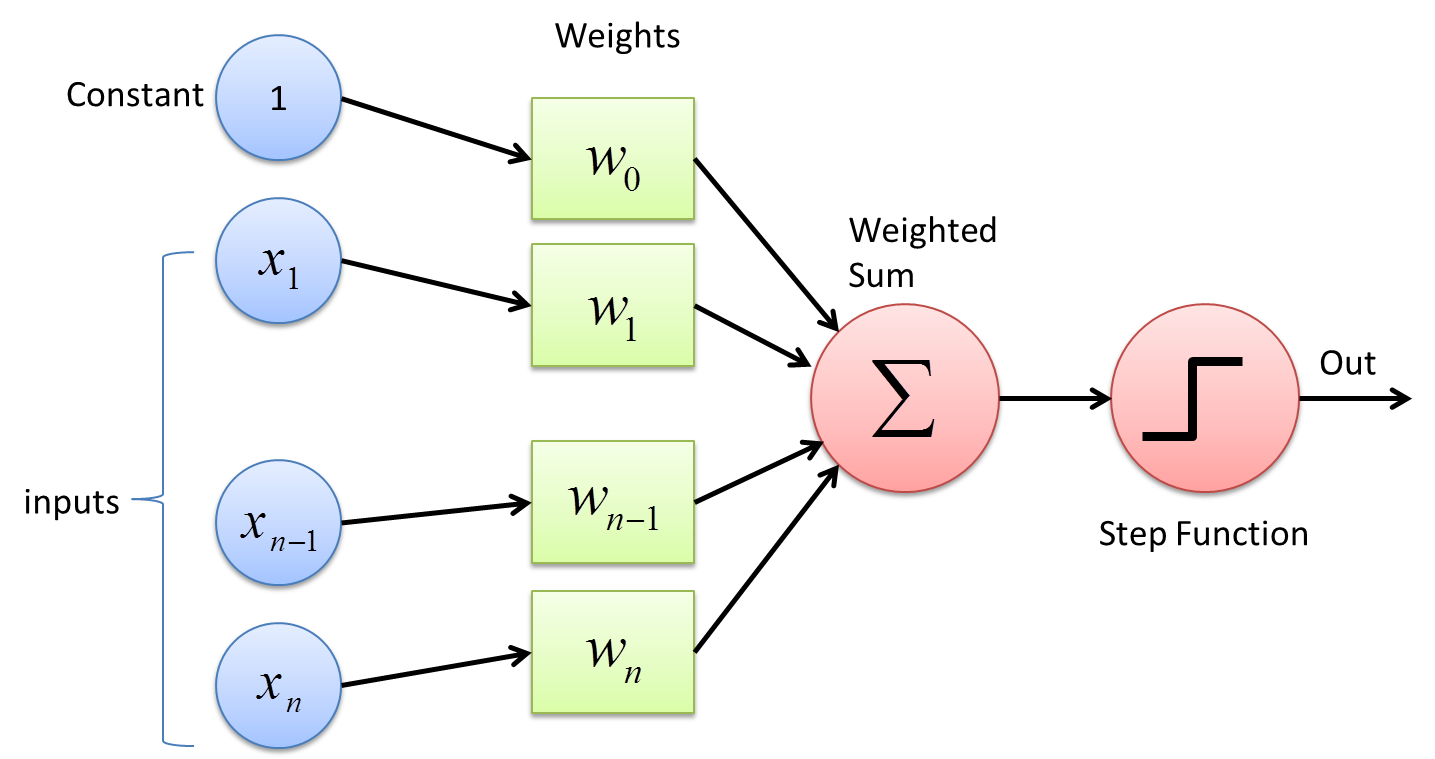
\includegraphics[scale=0.45]{images/perceptron-picture.png}
\caption{\cite{perceptron} Schematic illustration of a perceptron, the simplest Artificial Neural Network. Shown above are the initial stimuli which are then summed as weights and used as an input to an activation function.
This in turn will output either one of two classes. If it is wrong compared to the expected output, the weights are increased or decreased accordingly.}
\label{fig:perceptron}
\end{figure}
This report is not meant to be an indepth tutorial to machine learning so instead I shall take the approach to introduce only concepts vital to understanding what we produced and the methods by which we measure the value of our work. For a true introduction I strongly recommend \textit{Mehta et al.}'s review \cite{mehta2019high}.
\newline

The first important remark is that machine learning is a field generally focused more on predicting than estimating.
In this respect it is different from the classical statistical techniques and therefore different metrics must be used to assess its performance.
Estimation can be conceptualised with having knowledge about a particular experimental setup and trying to calculate its results as closely to our knowledge about the system.
Prediction on the other hand is understanding the results of this particular experiment and generalising them so as to be able to predict the results of new experimental setups.
Following from this, machine learning naturally splits into two : supervised and unsupervised learning \cite{Love2002}.
\newline

We can take the analogy of teaching a child to write the letter 'A'. A parent might take two approaches: Show many examples of a letter 'A' and after a number of examples ask the child to try themselves. Based on their output give appropriate feedback.
Otherwise, the parent could ask the child to draw something random and the closer or further they get each time to an 'A' give appropriate feedback.
\newline

One might note that in this analogy the second approach is needlessly complex and will take way too much time. This shows the nature of machine learning and how each approach has its own use case. The first approach is what is known as supervised machine learning (ML) and is commonly used where there is large availability of training data and is used in classification and pattern recognition problems. The second approach is an example of unsupervised learning and is used mostly on pattern recognition and generation from unlabelled datasets. The approach taken by us in our algorithms is of unsupervised learning.
\newline

The most general machine learning model is known as an Artificial Neural Network (ANN) \cite{ANN}.
This in turn divides into a myriad of particular neural networks but the simplest one is Rosenblatt’s perceptron \cite{rosenblatt1961principles} algorithm which dates back to early 1960s.
It is an example of supervised machine learning algorithm but it introduces most of the important and recurring concepts in ANNs. Figure \ref{fig:perceptron} illustrates such concepts.
\newline

Moving from left to right, stimuli drive the perceptron.
Weights are assigned to the inputs and aggregated into a weighted sum.
This in turn is used as an input to an activation function which is just a mapping chosen to reduce dimensionality to (usually) a binary classification.
In more complex systems the choice of the activation function is of paramount importance and in higher dimensionality problems the algorithm will only converge for a limited number of activation functions.
\begin{figure}[H]
\centering
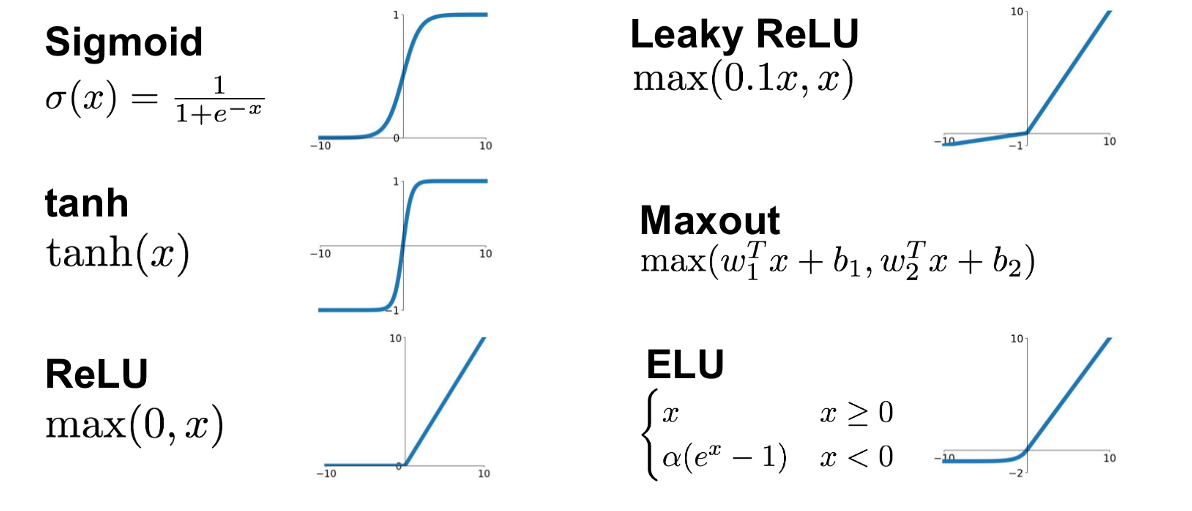
\includegraphics[scale=0.35]{images/activation_functions.png}
\caption{\cite{activationfuncs} Plots of some of the most common activation functions used in modern neural networks. In our algorithms we make use of Leaky and traditional ReLUs and Sigmoids.}
\label{fig:activation_functions}
\end{figure}

The output of the activation function is then compared to the expected output and if it is incorrect the weights are modified.
Generalising to other, more complex neural networks we need a metric of how good our classifier is and how 'wrong' the predicted class was from the expected one.
This is done by introducing an important concept known as the loss function. In all cases we want to minimise the value of the total loss.
\newline

Given a dataset of examples $ {( {x_i} , {y_i} )}_{i=1}^N $ where ${x_i}$ is a training data example and ${y_i}$ its respective label the total loss is defined as

\begin{equation}
L = \frac{1}{N}\sum_{i=1}^{N}{L_i}(f({x_i},w),{y_i})
\label{eq:totalLoss}
\end{equation}
where ${L_i}$ is the loss function used, $w$ are the weights and $f({x_i},w)$ is the activation function. There are different forms of the loss function and each has usually its use case \cite{zhao2015loss} but the one selected by us in our algorithms is categorical cross-entropy \cite{zhang2018generalized} which is a type of binary crossentropy where the 'categorical' part signifies that only one output can be correct. This is used usually in Generative Adverserial Networks since, as explained later, the aim for the adversary is to classify inputs as generated or real. This loss function has the form
\begin{equation}
{L_i} = -\hat{y_i}\log{(f({y_i},w))} - (1-\hat{y_i})\log{(1-f({y_i},w))}
\end{equation}
where $\hat{y_i}$ is the expected class label for the $i$'th element and $f({y_i},w)$ is the output of the activation function.
\newline

The aim is to always minimise the loss, so we need to compute the gradient of the weight vector $w$ as $L$ changes hence we need to find ${\nabla_w}$. Using the chain rule, the gradient of $w$ for each so called node of the neural network is calculated going from the final output of the activation function backwards and the weights are updated until we reach the original inputs (the stimuli). The weights are updated by the following pseudocode,
\begin{algorithm}
%\DontPrintSemicolon % Some LaTeX compilers require you to use \dontprintsemicolon    instead
\KwIn{Weights, Loss Function, Learning Rate}
\KwOut{Weights}
weightsGradient = evaluateGradient(lossFunction,weights)\\
weights = $-$learningRate * weightsGradient\\
Repeat \textit{Steps 1 and 2} until a maximum epoch number (hardcoded) is reached.
\caption{Pseudocode algorithm to minimise loss and update weights. This is known as the Stochastic Gradient Descent optimizer.}
\label{algo:minLoss}
\end{algorithm}
\newline
This will ensure we are always minimising the value of the loss. This last step is known as backpropagation (and is the backbone of machine learning) whilst the whole process up to this point is known as one epoch. The learning rate is also a very important parameter in such a simple machine learning algorithm since choosing it to be too large can make the problem impossible to converge and too small might mean the weights will take enormous amounts of time to converge. Tunable parameters such as learning rate are known as hyperparameters whilst parameters such as weights are tuned by the algorithm through backpropagation.
\newline

Lastly there are some problems about getting stuck on local minima in the gradient descent algorithm and strong dependence on initialisation. Furthermore, we should require that our algorithm minimises loss on test (unseen) data rather than be perfect on training data. The first problem is tackled through the introduction of a mathematical tool known as batch normalisation. It is a way to keep activations (outputs of nodes) as unit Gaussians. This is done by computing the empirical mean and variance
independently for each dimension $(k)$ of the input and normalising it by using

\begin{equation}
\hat{x}^{(k)} = \frac{{x^{(k)}}-E[{x^{(k)}}]}{\sqrt{Var[{x^{(k)}}]}}
\end{equation}

Hence, batch normalisation improves gradient flow, allows higher learning rates and reduces strong dependence on initialisation. In our algorithms we make use of this technique.
\newline

The second problem previously mentioned is tackled by a technique known as regularisation which in summary favours the simplest model that still minimises the total loss. It is a kind of bias added onto the total loss as a measure of simplicity of the model. A modified version of Equation \ref{eq:totalLoss} implements this as follows

\begin{equation}
L = \frac{1}{N}\sum_{i=1}^{N}{L_i}(f({x_i},w),{y_i}) + \lambda R(w)
\end{equation}
Batch normalisation is also an example of regularisation but another example often used in our algorithms this semester is known as dropout. The idea is that at each epoch, some nodes are blocked from being activated thus implementing a sort of stochasticity in the system and might prevent the algorithm from getting stuck at a local minimum. Other examples of regularisation are max norm and stochastic depth.
\newline

Algorithm \ref{algo:minLoss} is pseudocode for the stochastic gradient descent (SGD) algorithm. More technically this step is know as optimization and SGD is known as an optimizer. However it is subject to failure for high condition numbers (the ratio of smallest to largest singular value of the Hessian matrix being large). This means loss changes quickly in one direction and slowly in the other forming a sort of 'zigzag' optimization path which means very slow progress in converging along the less sensitive dimension. Local minima and saddle points are also a bane of this optimizer and the latter are much more common in higher dimension problems, so we need another optimizer to tackle these issues.
\newline

Thankfully, another optimizer which is the product of lots of work and many iterations of older optimizers is called Adam \cite{kingma2014adam}. It makes use of moments in its optimization and build up 'velocity' as a running mean of gradients. It also uses the idea of biases to prevent the first step from being too large and therefore the algorithm never converging. Finally, it has a decay rate on the learning rate itself which means the algorithm will train more precisely with time or epochs passed.
\newline

\begin{algorithm}
%\DontPrintSemicolon % Some LaTeX compilers require you to use \dontprintsemicolon    instead
\KwIn{Weights, Loss Function, Learning Rate, ${\beta_1}$, ${\beta_2}$, t (current iteration number)}
\KwOut{Weights}
weightsGradient = evaluateGradient(lossFunction,weights)\\
firstMoment = ${\beta_1}$*firstMoment+(1-${\beta_1}$)*weightsGradient\\
secondMoment = ${\beta_2}$*secondMoment+(1-${\beta_2}$)*weightsGradient$^2$\\
firstBias = firstMoment/(1-${{\beta_1}^t}$)\\
secondBias = secondMoment/(1-${{\beta_2}^t}$)\\
weights -= learningRate * firstBias / (+${10^{-7}}$) \\
Repeat \textit{Steps 1 to 6} until a maximum epoch number (hardcoded) is reached.
\caption{Pseudocode for the Adam optimizer as a substitute for the SGD optimizer.}
\label{algo:adam}
\end{algorithm}

Finally combining all of these steps mentioned, placing many layers in series and running it for numerous epochs is what a modern neural network looks like. Plots of accuracy and loss are vital since they are visible parameters which measure performance and can highlight if the algorithm will converge or not. After an arbitrary number of epochs it is customary to run a single run of the algorithm on unseen data and looking at the result. As will be seen later on, we do this particularly since we are generating distributions and overlaying them with the G4DS simulation distribution really helps in deciding if we need to vary or not the hyperparameters.

\subsubsection{Generative Adverserial Networks (GANs)}
\begin{figure}[H]
\centering
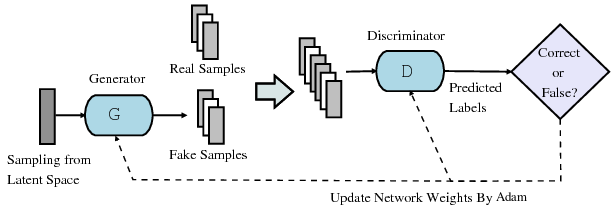
\includegraphics[scale=0.7]{images/gans.png}
\caption{\cite{Plakias2018GenerativeAN} Schematic of a GAN.}
\label{fig:gan_schematic}
\end{figure}

In 2014 a revolutionary paper \cite{NIPS2014_5423} was published proposing a new architecture of deep neural networks linked with each other. It hypothesised the use of two neural networks, one known as a discriminator and one known as a generator. They are interlinked via their losses since the loss of one is the accuracy of the other. The original version of this had a few problems which were later tackled by a 2016 paper \cite{salimans2016improved}.
\newline
The inescapable analogy in most literature is that of a forger and an expert critic. Assume there is a forger who wants to fake paintings of Vincent Van Gogh. Starting from random inspiration they paint on a canvas and present it to a critic. The latter immediately recognizes it as a fake and gains respect amongst the art community while the forger loses respect. The forger then takes the random inspiration they started with and works on it to produce yet another painting. This is closer to the original painter's but still rather wrong and the critic, although a bit less confident, decries the fake. This back and forth is carried out many times until the paintings made by the forger are indistinguishable by the critic who knows no better than a 50\%-50\% probability that the painting might be fake.
\newline

Although this might sound like a humorous but unrelated analogy it is almost identical to how GANs work in practice and the example mentioned was really implemented \cite{vangogh} as a GAN. The generator is a neural network which starts with a random noise vector and at each epoch generates a distribution which is passed to the discriminator. This in turn is a binary classifier to decide between real and fake. The generator's loss is related to the discriminator's accuracy therefore linking the two. The aim therefore is to make the generator create distributions indistinguishable from the training dataset and the discriminator to have about 50\% accuracy and about 70\% loss.
\newline

Finally, there exists an extension to GANs known as conditional GANs (cGANs). These are algorithms that together with starting from random noise take an additional input vector known as the condition. In the case of our project this would be the recoil energy of the distribution we want the GAN to learn. This is done such that after training we can give an arbitrary energy to the cGAN and it will produce a distribution specific for that energy. This adds an extra layer of difficulty in training since now the GAN is expected to learn the distribution but also the relationship between the input condition and the distribution itself.

\section{Methods and Results}
\subsection{Workflow and environment}
For coding all the machine learning algorithms we worked on a multi-user jupyter notebook style cloud service provided by Google called Colab. Its free plan provides access to 100Gb of storage, 12Gb of RAM and use of NVIDIA T4 GPUs designed for training of machine learning algorithms. We decided to use a prepared framework for machine learning in python called Tensorflow which is made by Google. Moreover, we used a further layer of abstraction on top of it called Keras which makes putting objects such as optimizers and layers together in one or two lines.
\subsection{1D GANs}
\subsubsection{Non-Conditional Case}
\begin{figure}[H]
\centering
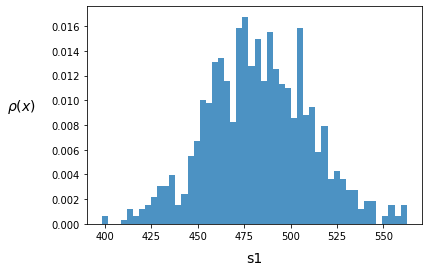
\includegraphics[scale=0.4]{images/1d_s1_simulation.png}
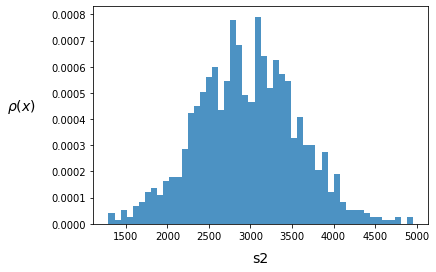
\includegraphics[scale=0.4]{images/1d_s2_simulation.png}
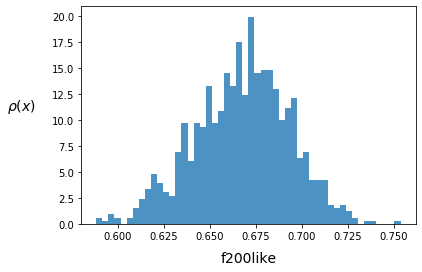
\includegraphics[scale=0.4]{images/1d_f200_simulation.png}
\caption{These are the distributions for $S1$, $S2$ and $f_{200}$ TPC responses obtained from the G4DS simulations for 50 keV Ar40 nuclear recoils, which are what a WIMP interaction would look like as shown in Figure \ref{fig:variablesExamples}. }
\label{fig:1DG4DS}
\end{figure}

The first distributions we tried to recreate were single variable for an arbitrary (but still theoretically sound) energy Ar40 nuclear recoils, in this case 50 keV. As explained previously we trained independently on $S1$, $S2$ and $f_{200}$. For this problem, but also extending to what we found for higher dimensions, the best approach is to start from a simple architecture and then add on more layers and nodes. The distributions we wanted to reproduce are seen in Figure \ref{fig:1DG4DS}.
\newline
\begin{figure}[H]
\centering
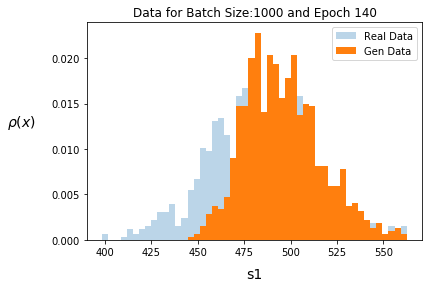
\includegraphics[scale=0.45]{images/1d_s1.png}
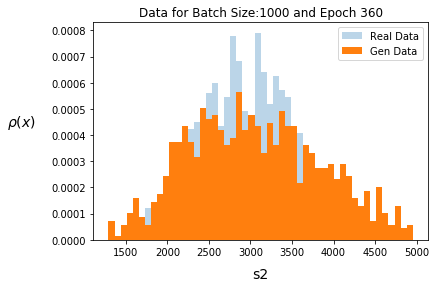
\includegraphics[scale=0.45]{images/1d_s2.png}
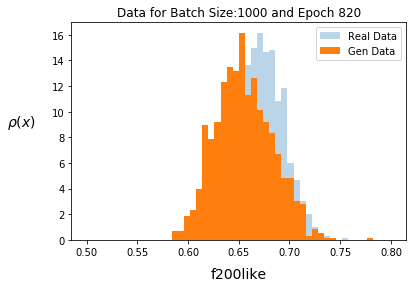
\includegraphics[scale=0.45]{images/1d_f200.png}
\caption{Overlayed plots showing the GAN learning to reproduce the shape of the distributions correctly. The lighter plots are G4DS simulation data while the bright plots are generated by the GAN.}
\label{fig:1DGAN}
\end{figure}

From this GAN we learnt that to help it converge sooner and also for it to be able to work with little to no modification for all three variables we needed a level of data preprocessing. We normalised the distribution by dividing it by the largest value in the dataset and multiplied it back at the end of training. We also learnt that batch normalisation is very easily misused and can make the GAN appear to not converge when in fact simply removing the batch normalisation solved the issue. There is indication \cite{ioffe2015batch} that this tool is rather new and still far away from actually being fully understood so more research needs to be carried out using this technique before we can use it with confidence.
\newline

On a more practical note, the GAN that seems to work as seen in Figure \ref{fig:1DGAN} has close to 10,200 trainable parameters and both neural networks with equal number of layers and nodes. One thing to mention is that although the plots show room for improvement, this is only due to us stopping the GAN after a number of arbitrary epochs when it was clear the generator had got a clear idea of what the distribution looked like. As I mentioned before, we still do not have a clear metric to classify how 'good' the GAN performs. That is more a focus of the second semester and for now visual aid of seeing the generated plots together with the loss graph as shown in Figure \ref{fig:1DGANLoss} gives a reasonably good metric. Also important to note that the neural network was not changed between different variables indicating that the particular neural network works well for that kind of distribution.

\begin{figure}[H]
\centering
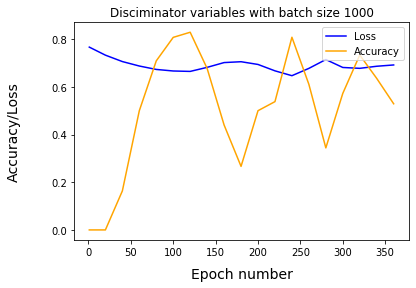
\includegraphics[scale=0.5]{images/1d_loss_graph_s2.png}
\caption{A graph of loss/accuracy of the discriminator as training $S2$ whose final result is shown in Figure \ref{fig:1DGAN}. Note the initial turbulent behaviour which oscillates with decaying intensity around an accuracy of 50\% and stable loss of about 70\%.}
\label{fig:1DGANLoss}
\end{figure}
\subsubsection{Conditional Case}
The next step was to give the GAN the energy of the distribution being trained on as a condition. After training, we could then provide the GAN with an arbitrary energy \textbf{not in the training dataset} and see its performance compared to simulation data. For this step we used 50 keV, 100 keV and 150 keV recoil energies. Figure \ref{fig:1DcGAN} shows the results of such cGAN.

\begin{figure}[H]
\centering
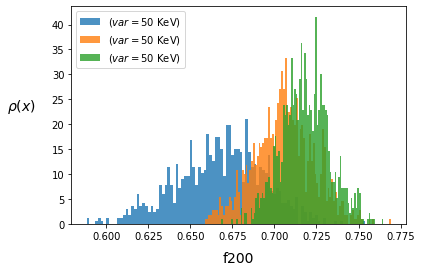
\includegraphics[scale=0.45]{images/1d_conditional_f200_simulation.png}
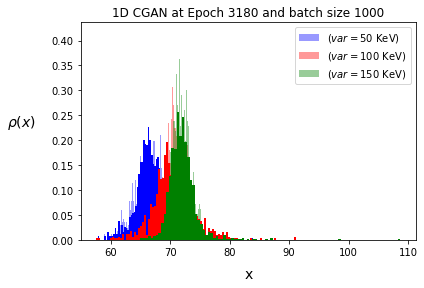
\includegraphics[scale=0.45]{images/1d_conditional_f200.png}
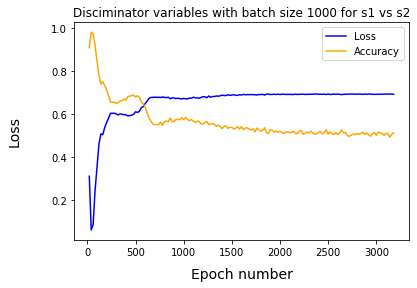
\includegraphics[scale=0.45]{images/1d_conditional_loss_f200.png}
\caption{Top Left: The $f_{200}$ variable from simulation to be learnt by the algorithm. Top Right: A plot of generated and simulation distributions. Bottom: The accuracy/loss curve which shows very good results.}
\label{fig:1DcGAN}
\end{figure}

As one can see from how well the distributions fit the data together with the loss/accuracy graph, the results are very promising. I choose the word promising however since it is also clear there is room for improvement. Looking at the red distribution in Figure \ref{fig:1DcGAN} which represents a 100 keV recoil, the GAN produces a distribution which is similar but with a mean to the left of the real one and more spread out.
\newline

However, as I mentioned before, the real test for such a cGAN is providing an energy which was not part of training and observing the results compared to simulation data. In Figure \ref{fig:1DcGANtest} we used an input of 125 keV into the condition vector and the results again are very promising. The shape, mean and scale of the distributions are very similar.

\begin{figure}[H]
\centering
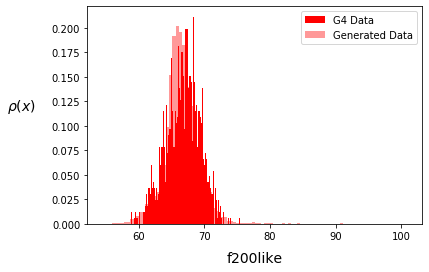
\includegraphics[scale=0.5]{images/1d_conditional_f200_50kev.png}
\caption{Inputting 125keV as an input condition, which is an unseen energy to the cGAN, it reproduces the G4DS data very well.}
\label{fig:1DcGANtest}
\end{figure}

This test however proved to be even more important since we noticed something very interesting. On trying to provide it with 200 keV as a condition, which is \textbf{outside of its training range} the GAN fails. As can be seen from Figure \ref{fig:1DcGANfailure} (right) all the properties such as shape, mean and spread are all wrong. This was a good point for us to further analyse and on attempting 75 keV, seen in the same Figure \ref{fig:1DcGANfailure} (left), the GAN produced a distribution which is not great at all. The mean is too to the left and the spread is also not similar to the simulations with the generated distribution even having two peaks.
\begin{figure}[H]
\centering
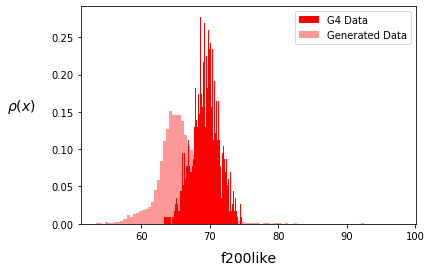
\includegraphics[scale=0.5]{images/1d_conditional_f200_75kev.png}
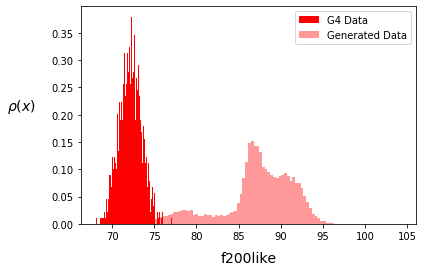
\includegraphics[scale=0.5]{images/1d_conditional_f200_200kev.png}
\caption{(Left) On 75 keV as a condition the cGAN starts to fail to recreate simulation data. (Right) Outside of its training range for 200 keV the cGAN completely fails to recreate simulation data and highlights the need for further analysis of this failure.}
\label{fig:1DcGANfailure}
\end{figure}

This seems to show that the GAN is better at interpolating than extrapolating and further testing is required in the second semester to take this into account when choosing what energies to train on. We might realise we require fewer points but more spread out for the cGAN to really be able to reproduce the simulations properly. One thing we decided after this was that we should include these checks as the GAN is training. Every arbitrary number of epochs the GAN produces a distribution for an energy not in the training dataset and checks how good it can fit simulations. This 'custom-made' loss function is described by Equation \ref{eq:customloss} and although simple in nature seemed to work as intended. Here, $\hat{h}_i$ is the $i$'th bin in the simulation distribution and ${h_i}$ is the $i$'th bin in the generated distribution. It then saves the current weights only if the current score is less (a better fit) than the previous ones. This ensures that the stochastic nature of the GAN does not mean we find the minimum and then 'lose' it later on in training. In the second semester we will try to work more on this and focus on reproducibility of results while still retaining the stochastic nature of the GAN.

\begin{equation}
L = \sum_{i=1}^{N}{\lvert{\hat{h}_i}-{h_i}\rvert}
\label{eq:customloss}
\end{equation}

\subsection{2D GANs}
\subsubsection{Non-Conditional Case}
Due to the promising results of the 1D GAN we decided to investigate how different training a 2D GAN is. The network we used is very similar to the one for the 1D GAN however we needed to increase the number of trainable parameters to 100,000. The results are shown in Figure \ref{fig:2DGAN} and again are very promising. We trained it for 100 keV recoil events on a 2D scatter plot of $S1$ vs $S2$. As mentioned before we preprocessed the data by normalising it to be able to reuse the same network for different energies later on.

\begin{figure}[H]
\centering
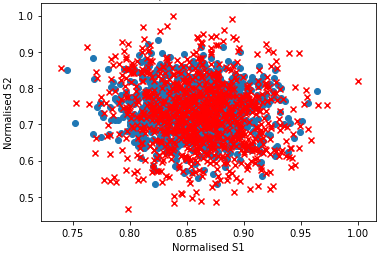
\includegraphics[scale=0.7]{images/2d_s1_s2_1600.png}
\caption{Results of training after 1600 epochs on a 2D scatter plot of $S1$ vs $S2$ for 100 keV recoils. Red crosses are from G4 simulation data  and the blue circles are generated by the GAN.}
\label{fig:2DGAN}
\end{figure}

The real test after this was to check the individual $S1$ and $S2$ distributions and check how well the simulation data overlapped the generated data. These are shown in Figure \ref{fig:2DGANindividual}. Both generated distributions look very similar to the ones from G4DS and this was confirmed for other energies, namely, 50 keV and 150 keV.

\begin{figure}[H]
\centering
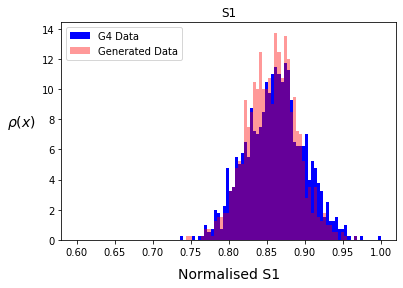
\includegraphics[scale=0.55]{images/2d_s1.png}
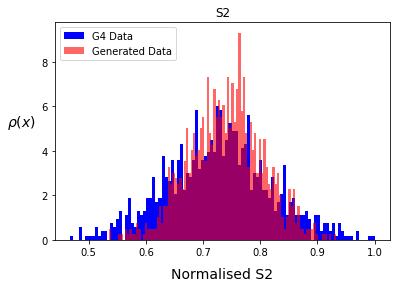
\includegraphics[scale=0.55]{images/2d_s2.png}
\caption{Individual normalised $S1$ and $S2$ distributions showing a good generation by the GAN. Features such as mean, shape and spread are all correctly modelled by the GAN.}
\label{fig:2DGANindividual}
\end{figure}

One final measure of how well the GAN is training is as always the loss/accuracy curve. Figure \ref{fig:2DGANloss} shows such a curve and this confirms the positive results we observed in previous figures.

\begin{figure}[H]
\centering
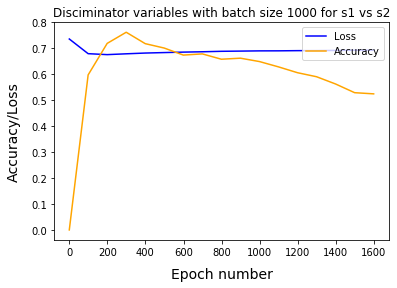
\includegraphics[scale=0.6]{images/2d_loss_graph_s1_s2.png}
\caption{Loss/Accuracy curve of the 2D GAN confirming the stable model that reproduces the training curves.}
\label{fig:2DGANloss}
\end{figure}

\subsubsection{Conditional Case}

Finally, we arrive at the true aim of this semester's work: To produce a 2D cGAN that can reproduce variables of importance such as $S1$ and $S2$ on condition of recoil energy. For training, like in the 1D cGAN we used 50, 100 and 150 keV recoil energies. As a test dataset we used a 200 keV recoil energy and as mentioned before, at each 200 epochs the GAN would produce a 200 keV distribution, compare it using Equation \ref{eq:customloss} and save the weights only if it fits the test case better. This allowed us to save the best model for that particular run as can be seen by the very good results in Figure \ref{fig:2DcGAN}. The most important feature is that although the cGAN does not exactly model the three simulation distributions it still very well describes the 200 keV distribution which was not part of training but was part of the testing.

\begin{figure}[H]
\centering
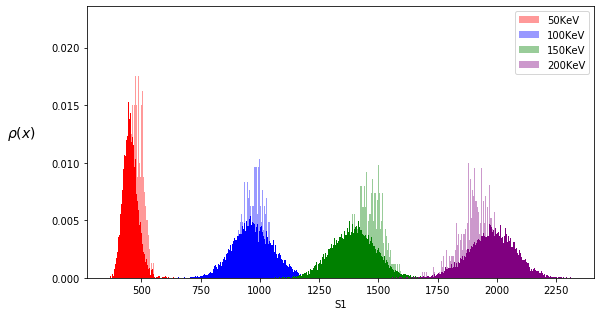
\includegraphics[scale=0.6]{images/2d_conditional_s1.png}
\linebreak
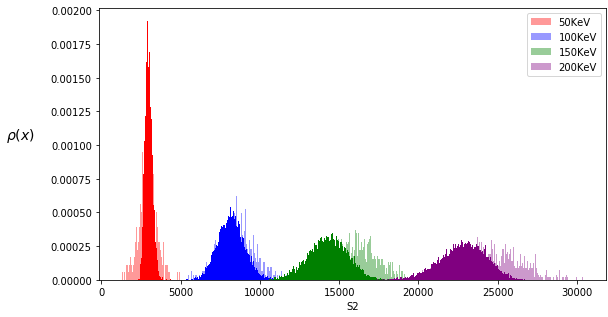
\includegraphics[scale=0.6]{images/2d_conditional_s2.png}
\caption{Results of the best performing cGAN run out of 15000 epochs. At the top is the $S1$ distribution whilst at the bottom is the $S2$ distribution. The bright coloured distributions are generated by the cGAN while the more transparent ones are from G4DS simulations. The purple distribution is for an unseen 200 keV recoil energy not part of the training which shows good flexibility of the cGAN.}
\label{fig:2DcGAN}
\end{figure}

Due to the complexity of the 2D cGAN (the network has 200,000 trainable parameters) and the length of time it therefore takes to train it (15000 epochs to get good results), we have not yet analysed it fully. Although preliminary results give us insight that our methods are on the right track, there is yet a lot of work to be done. One thing we did notice however is that from the output of distributions during training it seems like the cGAN will try to fit one parameter first, such as $S1$, and then focus on fitting the other. This is a feature of training that intrigued us, and we hope to investigate it further in the second part of this project.

\section{Final Remarks}

The past semester's work has provided us with really great foundations for the second one. We have started to narrow down the steps needed to train a GAN and even better, a cGAN. Following from our work it is clear we would like to successfully train a 3D cGAN on the variables $S1$, $S2$ and $f_{200}$. Doing this would allow us to produce plots for other variables and really be able to \textbf{quantitatively} compare our networks' output to G4DS simulations and real detector measurements.
\newline

This is actually a very important part of second semester's aims: To create a framework with which further studies could properly compare simulation and GAN output together with network-network comparisons. A possible means to achieve this is the use of a Wasserstein GAN \cite{arjovsky2017wasserstein} which takes a non-traditional approach to the discriminatory element of a GAN and its use of novel loss functions. This would help us create proper metrics which will be able to clearly discriminate between networks that match simulations and ones which do not.
\newline

Finally, we would like to also think of new and better visualisations of the variables we investigate. As we increase the number of dimensions and also energies for one particular dimension (the condition) we need to find new ways to visualise everything. This is to prevent clutter in presentation of our findings but furthermore we could perhaps find a representation which the GAN will find easier to train on. We have observed many times in this research that GANs are susceptible to the way we provide the input therefore finding different ways could help the model converge faster or even at all in cases where we could not previously.
\newline

Related to the experimental links to dark matter and neutrino serach we would like to expand on our work and research the use of GANs for directionality \cite{mayet2016review} prediction. This part has been subject to debate between my colleague and I but also with our supervisors, and we are still deciding if and how we shall do it. Even relatively little knowledge on directionality could be very beneficial (such as which hemisphere the WIMP is coming from) to the collaboration. Technically speaking, this would probably be an additional module in the form of an encoder which works on the output of the GAN.
\newline



\newpage
\printbibliography

\end{document}
